\chapter{Grundlagen}
\label{Grundlagen}

\section{Datenbankverwaltungssysteme}

Eine der wichtigsten Aspekte einer Datenbankanwendung ist die Performance. 

Mit der Zeit wird es auf der Welt bedeutsamer, große Mengen an Daten, mithilfe einer Datenbank, persistieren und verarbeiten zu können.\cite{Memory:Usage}
In Bezug auf den Speicher kann hier unterschieden werden zwischen einer In-Memory Datenbank, wie beispielsweise Redis \cite{Redis} oder H2 \cite{H2} und einer On-Disk Datenbank, wie Postgresql \cite{PostgreSQL}, die auf dem Sekundärspeicher operiert. \\

In-Memory Datenbanken haben den Vorteil, dass diese eine geringe Latenz bei Anfragen und Operationen vorweisen, da die Daten sich schon im Hauptspeicher befinden. Bei einer On-Disk Datenbank muss der benötigte Speicher bei einer Anfrage erst in den Hauptspeicher aus dem Sekundärspeicher geladen werden. Diese Input/Output Operationen konsumieren eine Menge Zeit bei einer großen Menge von Daten.\cite{KABAKUS2017520}
Aufgrund dieser Tatsache ist es für diese Thesis sinnvoll sich In-Memory Datenbankverwaltungssystem genauer anzuschauen. 
Vorerst muss jedoch geklärt werden, welche Arten es von Hauptspeichern gibt und welche Speichertechnologien die Zukunft mit sich bringt.

\section{Speichertechnologie}

\subsection{Hauptspeicherarten}

Es gibt mehrere Arten von Hauptspeicher. Eine der gängigsten Arten sind Dynamic Random Memory Access, abgekürzt DRAM, und Static Random Memory Access, abgekürzt SRAM.Im Gegensatz zu DRAM ist SRAM deutlich teurer, da es um ein Datenbit zu halten, mehrere Transistoren benötigt. Jedoch steht SRAM gegenüber DRAM Performance-technisch in Bezug auf die Geschwindigkeit besser dar.\cite{techtarget:Ram}

\subsection{Neue Speichertechnologie}
Durch die immer größer und immer schneller werdende Entwicklung von digitalen Medien und Dienstleistungen, steigt auch die Größe an produzierten Daten. 
Das Unternehmen Intel publizierte 2015 einen Artikel \glqq{}Intel and Micron Produce Breathrough Memory Technology\grqq{}, in dem sie die Erfindung der \glqq{}3D Xpoint\grqq{} Technology bekannt gaben. Diese Technologie brachte eine neue Speicherkategorie auf den Markt. Es handelt sich hierbei um nicht flüchtigen Speicher, der 1000 mal schneller sein kann, als der gängige Sekundärspeicher. \cite{Intel:MemoryTechnology}

Mit diesem Artikel kam die Hardware Intel Optane Persistent Memory auf den Markt, der eine Kapazität von bis zu 512 GB an Speicher aufweisen kann.
Im Gegensatz dazu befindet sich DRAM bei ca 128GB.
Diese neuen Speichermodule sind DDR4 kompatibel und somit als Hauptspeicher nutzbar. \cite{IntelOptane:Micron}

Gegenüber DRAM hat das Intel-Optane-Modul Nicht-flüchtigen Speicher. Das bedeutet, dass  Daten, die sich in einer Datenbankverwaltung befinden, bei Spannungsverlust nicht verloren gehen.
Die Eigenschaften des Intel-Optane Moduls sollen es ermöglichen, eine Große Menge an Daten im Speicher abzulegen und trotz der Verwendung von Nicht-flüchtigem Speicher eine gute Performance sicherzustellen.
 
\subsection{Reihen-orientierter Speicher vs Spalten-orientierter Speicher}
Es spielt für die Performance, eine große Rolle, in welchem Format die Daten in den Speicher gelegt werden. Hier wird unterschieden zwischen dem Reihen-orientierten und dem Spalten-orientierten Speicherformat.
Die meisten traditionellen Datenbankverwaltungssysteme benutzen ein Reihen-orientiertes Speicherformat,das Datentupel aus den Reihen hintereinander im Speicher persistiert. Solch ein System ist laut \cite{Stonebraker2005CStoreAC} ein \glqq{}Schreib-optimiertes System\grqq{}.

Bei einem Spalte-orientierten Datenbanksystem, werden keine Datentupel hintereinander im Speicher persistiert, sondern die Einträge spaltenweise nacheinander pro Eintrag, in den Speicher gelegt. Die Grafik \ref{graf_8} zeigt, dass jeder Eintrag einer Spalte, hintereinander im Speicher liegt. Auf diese Weise, können auf größeren Datensätzen schnellere Funktionen auf einzelne Einträge ausgeführt werden, ohne dass Daten, die nicht benötigt werden, mitgeladen werden müssen.

\begin{figure}[h]
  \centering
  \begin{subfigure}[b]{0.5\textwidth}
    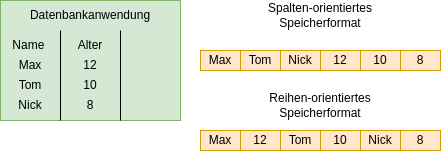
\includegraphics[width=1.0\linewidth]{img/speicher}
  \end{subfigure}
  \caption{Reihen-Orientiert vs Spalten-Orientiert}
  \label{graf_8}
\end{figure}

Da die Daten eines Objektes hier Spaltenweise persistiert werden, können Operationen auf langen Spalten sehr performant ausgeführt werden.
Aufgrund dieser Vorteile wird in dieser Arbeit ausschließlich eine In-Memory Datenbank mit einem Spalten-orientierten Speicher behandelt.
Zur Speicherung der Daten in einem Spalten-orientierten Format wird Apache Arrow verwendet.

\section{Apache Arrow}

Apache Arrow ist ein Framework, das ein Sprachen-unabhängiges Spalten-orientiertes Speicherformat definiert. 
Um Arrow nutzen zu können, stellt Apache, in verschiedene Sprachen Bindings zu Verfügung. In dieser Arbeit wird die Programmiersprache Java benutzt, und daher ist die Dokumentation der Java-API von Apache Arrow eine wichtige Informationsquelle.\cite{Apache:Arrow:JavaApi}\\
Arrow umgeht das Problem, dass jede Sprache eine unterschiedliche Serialisierung und Deserialisierung von Daten im Speicher und in der Übertragung von Daten über das Netzwerk, unterstützt.
Das Framework vereinheitlicht die Serialisierung und Deserialisierung, indem es sämtliche Objekte unter der Haube als Datenstrom interpretiert. Dies bedeutet, dass Anwendungen, die das Arrow Format verstehen, Daten mittels geringer Kosten übertragen können.\cite{Arrow:overview}
Im folgenden Teil wird auf die verschiedenen Mechanismen und Prinzipien zur Speicherung von Daten, mithilfe des Arrow-Frameworks eingegangen. Dazu werden verschiedene Klassen beschrieben und Beispiele erklärt.


\subsection{Vektoren in Arrow}
Vektoren können in Arrow verschiedene Typen von Daten halten. Beispielsweise gibt es die Klasse \texttt{IntVector} oder \texttt{VarCharVector}.
Der \texttt{IntVector} basiert auf der Klasse \texttt{BasedFixedWidthVector} und stellt einen Vektor dar, der eine feste Größe an Bytes besitzt. Jede Art von Vektor besitzt unter der Haube einen Werte-Buffer und einen Validierungs-Buffer in Form eines \texttt{ArrowBuf}-Objektes.\\
Mithilfe dieser Buffer ist es möglich Daten zu allozieren und schneller auszuwerten. Warum können diese schneller ausgewertet werden?
Weil Arrow mithilfe des Validierungs-Buffers, Dateneinträge im Vektor überwacht, welche ein null-Objekt repräsentieren könnten. Diese würden aufgrund des Buffers bei einer Evaluierung nicht mit ausgewertet werden. Ebenfalls kommt hier der Faktor des Spalten-orientierten Formats zu Tragen.

Ein Beispiel kann aus der Dokumentation \cite{Apache:Arrow:ValueVector} entnommen werden.

\label{VectorValue}
\begin{codeblock}{ValueVectorBeispiel.java}{Java}
  \begin{javacode}

RootAllocator allocator = new RootAllocator(Long.MAX_VALUE);
...
IntVector vector = new IntVector("int vector", allocator);
vector.allocateNew(10);
vector.set(/*index*/5, /*value*/25);
vector.setValueCount(10);
int value = vector.get(5); 
vector.close();
  \end{javacode}
\end{codeblock}

In dem Code-Beispiel \ref{VectorValue} wird die Allokation eines Integer-Vektors dargestellt. Einem Vektor wird im Konstruktor ein Name übergeben und ein \texttt{Allocator}, der sicherstellt, dass die Daten im Hauptspeicher zur Verfügung stehen.
Mit der Methode \texttt{set(int index,int value)} kann an eine Stelle im Vektor ein Wert eingetragen und gespeichert werden.
Dieser kann mit der Methode \texttt{get(int index)} wieder aufgerufen werden.


\subsection{VectorSchemaRoot}

Die Klasse \texttt{VectorSchemaRoot} dient in Arrow, als eine Art Container-Klasse für Vektoren. \texttt{VectorSchemaRoot} benötigt ein Schema, um Vektoren innerhalb der Klasse zu befüllen.
Meist kann es ausreichen nur eine \texttt{VectorSchemaRoot}-Instanz zu initialisieren, da in diesem beliebige Vektoren gefüllt und gelöscht werden können.
In dieser Arbeit ist dem \texttt{VectorSchemaRoot}-Objekt viel Aufmerksamkeit zu schenken, da es zur Speicherung der Datenbankeinträge verwendet wird.

\texttt{VectorSchemaRoot} besitzt eine statische Methode \texttt{create(Schema schema, Allocator allocator)} mit der eine Instanziierung möglich ist.
Nachdem das Objekt instanziiert wurde, kann mithilfe der Methode \texttt{getVector(String vektorName)} auf den leeren Vektor, wie in \texttt{VectorSchemaRootBeispiel.java}, zugegriffen werden.

\begin{codeblock}{VectorSchemaRootBeispiel.java}{Java}
  \begin{javacode}
...
IntVector intVector = vectorSchemaRoot.getVector(vektorName);
intVector.set(1,200);
...
  \end{javacode}
\end{codeblock}


Hier hält das \texttt{VectorSchemaRoot}-Objekt, nun einen \texttt{IntVector} mit Wert 200 am Index 1 im Hauptspeicher.
Dieses Vorgehen ist nicht nur mit Integer-Vektoren möglich, sondern mit allen beliebigen Arten von Datentypen.


\section{Gandiva}
\label{Gandiva}
Das Open-Source Gandiva-Framework existiert grundlegend aus  einen Runtime-Expression-Compiler, der auf dem LLVM Projekt basiert, sowie eine hoch hochperformante Laufzeitumgebung.
Gandiva unterstützt Arrow bei dem Ausführen von Analytischen Funktionen auf Daten, die in einem Arrow-Format gespeichert sind. 
Das Framework wurde ursprünglich von dem Unternehmen Dremio entwickelt, das dieses jedoch an das Apache Arrow Projekt übergeben hat.\cite{Apache:Gandiva}

\subsection{Wie funktioniert Gandiva unter der Haube?}
Angenommen es existiert eine Anwendung, welche Daten mithilfe des  Apache Arrow-Frameworks verarbeitet.Je nach Anforderung dieser Anwendung, wird ein Ausdrucks-Baum (engl. Expression Tree) mithilfe von Gandiva-Klassen erstellt. Dieser Ausdrucksbaum wird nun intern von Gandiva in nativen Code, der für die Laufzeitumgebung und Hardware benötigt wird, übersetzt. \\
Gandiva ist mithilfe von Apache Arrow in der Lage, verschiedene, im Arrow-Spalten-Format abgelegte Daten, weiterzuverarbeiten, zu filtern und auszuwerten.
Dieser Prozess verläuft hoch optimisiert auf modernen CPU's.\cite{Apache:Gandiva} \\
Im August 2018 ist es den Ingenieuren von Dremio gelungen, eine SQL-Abfrage 70x schneller mithilfe von Gandiva zu verarbeiten. Diese Optimierung ist auf den LLVM-basierten Compiler und das Arrow Spalten-Format zurückzuführen.\cite{Apache:Gandiva:Performance}

\newpage

\subsection{Beispiel eines Filters}
\label{Beispiel eines Filters}

Da in dieser Arbeit die Datenbankanwendung mit der Programmiersprache Java umgesetzt wurde, wird hier auf den Java-Wrapper für Gandiva eingegangen.\\
Grundsätzlich wird mit Gandiva ein Ausdruck in Form von TreeNodes aufgebaut. TreeNodes ist ein Interface aus dem Package \textbf{org.apache.arrow.gandiva.expression}. Es gibt viele verschiedene Klassen für verschiedene Ausdrücke, die das TreeNode-Interface implementieren. 
Beispielsweise gibt es die Klasse \texttt{AndNode}, mit der sich einzelne Ausdrücke verknüpfen lassen.
Eine der wichtigen Klassen zum Bauen eines Ausdrucks ist die \texttt{TreeBuilder}-Klasse.

\subsubsection{TreeNode-Literal}
Mithilfe dieser Klasse ist es möglich, beispielsweise \texttt{TreeNode}-Literale aus verschiedenen Datentypen zu erstellen. TreeNode-Literale spiegeln einfach nur einen Wert wider, wie zum Beispiel einen Integer vom Wert fünf oder einen Double vom Wert 5.0. \\

\subsubsection{TreeNode-Field}
Das \texttt{Field}-TreeNode bildet den Typ des Vektors bzw. der Spalte der Datenbankanwendung ab und lässt sich ebenfalls über den TreeBuilder mit der Methode \textbf{makeField(Field field)} erstellen.
Die Field-Klasse beschreibt lediglich den Namen der Spalte und den Typ.

\subsubsection{TreeNode-Funktion}
\label{TreeNode-Funktion}
Ebenso lässt sich eine vollständige Funktion in Form eines TreeNodes darstellen.
Mithilfe des TreeBuilders lässt sich die Methode \texttt{makeFunction} aufrufen.

\begin{codeblock}{TreeBuilder.java}{Java}
  \begin{javacode}
    public static TreeNode makeFunction(String function, List<TreeNode> children, ArrowType retType) {
        return new FunctionNode(function, children, retType);
    }
  \end{javacode}
\end{codeblock}

Der, in der \texttt{TreeBuilder.java}, abgebildeten Funktion, wird ein Funktionsname in Form eines Strings übergeben (Zeile 2, TreeBuilder.java). Welche Auswahl es an vorgegeben Funktionsnamen gibt, muss jedoch manuell im Github-Repository nachgeschaut werden \cite{Github:Arrow:functionregistry}. In Abbildung \ref{graf_5} ist die Funktion \glqq{}equal\grqq{} in der Farbe gelb dargestellt. Diese ist eine von vielen bereits implementierten Funktionen im Gandiva Framework.\\

Ein weiterer Parameter in der Methode \texttt{makeFunction} ist eine Liste von TreeNodes.
In dieser Liste von TreeNodes befinden sich alle TreeNodes, die, der in dem String angegeben Funktion, übergeben wird.
In \ref{graf_5} wird verdeutlicht wie das Feld \glq{}Alter\grq{} und das Integer-Literal \glq{}5\grq{} miteinander durch die Funktion \glq{}equal\grq{} verglichen wird. \\
Schlussendlich wird ein Return-Type ausgewählt, der einen \texttt{ArrowType} abbildet. Mit dem \texttt{ArrowType} werden alle primitiven Datentypen, sowie weitere Datentypen wie \glqq{}List, Map, Time\grqq{} usw. abgedeckt.

\begin{figure}[h]
  \centering
  \begin{subfigure}[b]{0.5\textwidth}
    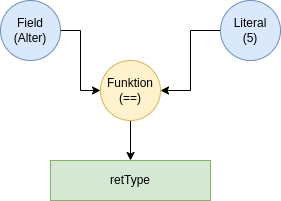
\includegraphics[width=1.0\linewidth]{img/gandiva_funktion}
  \end{subfigure}
  \caption{Gandiva TreeNode-Funktionsausdruck}
  \label{graf_5}
\end{figure}

\subsubsection{Filter}

Ein Filter benötigt zuerst ein \texttt{Schema}-Objekt, das aus einer Liste von \texttt{Field}-Objekten erstellt wird. Ebenso benötigt es ein \texttt{Condition}-TreeNode.
Hierzu muss wieder mithilfe der \texttt{TreeBuilder}-Klasse ein \texttt{Condition}-TreeNode mit einer Funktion, wie beispielsweise in \ref{TreeNode-Funktion}, erstellt werden.
Mithilfe des Filters können dann verschiedene \texttt{ArrowRecordBatche}'s evaluiert werden. Dies wird in \ref{GandivaProvider-Service} weiter erläutert.

\subsection{Motivation}

Mithilfe von Gandiva ist es möglich komplexe Abfragen von Daten zu strukturieren und durch eigene Ausdrücke auszuwerten. Da Gandiva mit dem TreeNode-Interface arbeitet, ist es möglich rekursiv, unendlich tiefe Ausdrücke zu generieren. In Bezug auf die Index-basierte Datenbankverwaltung lassen sich somit komplexe SQL-Anfragen durch Gandiva performativer verarbeiten, um so eine schnelle Antwort in Form von virtuellen Speicher-Adressen zu garantieren. 


\section{JSQL}

JSQL ist ein kleines Framework, das dazu dient SQL-Statements zu parsen und dieses dann in eine Hierarchie von Java-Klassen zu übersetzen.
Durch die erstellten Java-Klassen ist es dann möglich, mithilfe des Visitor-Pattern, durch diese zu navigieren und das Statement genauer zu betrachten.\cite{wumpz:JSQLParser} 
